% IE 643 novelty-assessment report (max 2 pages) -- Team Pensieve.
% Figures: scripts/make_novelty_figures.py -> report/novelty/figures/ (numbers copied from
% docs/experiments.md). The demo (Fig. 3) is report/novelty/demo_net.py; its two answers are the
% real output of graphart.extract.graph_from_code and graphart.hier.hier_from_code.
% Fig. 1 is the saved holdout reply of the final pipeline on tvh-mc3-bottleneck (closest of the 17
% by node and edge F1), drawn against its torch.fx truth; no model was re-run.
% Compile: latexmk -pdf Pensieve_IE643_NoveltyAssessment_report.tex
% Tags used across sections: D# = data set (Sec. 2), M# = method (Sec. 3), R# = result (Sec. 4).
\documentclass[10pt]{article}
\usepackage[a4paper,margin=0.42in,top=0.4in,bottom=0.4in]{geometry}
\usepackage[T1]{fontenc}
\usepackage{lmodern}
\usepackage{microtype}
\usepackage{graphicx,booktabs,tabularx,multicol,xcolor,array}
\usepackage[skip=1pt,font=footnotesize,labelfont=bf]{caption}
\usepackage[hidelinks]{hyperref}
\usepackage{enumitem}
\usepackage{listings}
\usepackage{tikz}
\usetikzlibrary{positioning,arrows.meta,fit,backgrounds}

\setlist{nosep,leftmargin=0.9em,label=\textbullet}
\setlength{\parindent}{0pt}
\setlength{\parskip}{1pt}
\setlength{\columnsep}{0.2in}
\setlength{\multicolsep}{2pt}
\pagestyle{empty}
\linespread{0.96}
\definecolor{tagc}{HTML}{2A78D6}
\definecolor{hiec}{HTML}{EB6834}
\definecolor{bad}{HTML}{E34948}
\newcommand{\tg}[1]{\textcolor{tagc}{\textbf{[#1]}}}
\newcommand{\sect}[1]{\vspace{1pt}{\large\bfseries #1}\par}
\newcommand{\sub}[1]{\vspace{1pt}{\bfseries #1}\par}
\newcommand{\demofont}{\fontsize{5.6}{6.3}\selectfont\ttfamily}
\lstset{language=Python, basicstyle=\demofont, columns=fullflexible, keepspaces=true,
  keywordstyle=\color{tagc}\bfseries, showstringspaces=false, frame=none, aboveskip=0pt, belowskip=0pt,
  xleftmargin=0pt}
\tikzset{fx/.style={draw, rounded corners=1.5pt, font=\fontsize{5.4}{6}\selectfont, inner sep=1.4pt,
  minimum height=3.6mm, minimum width=6.5mm, fill=white},
  sm/.style={fx, inner sep=0.9pt, minimum width=4.6mm},
  ar/.style={-{Stealth[length=3pt]}, line width=0.4pt}}

\begin{document}
\small

% ------------------------------------------------------------------ header
\noindent\fbox{\parbox{\dimexpr\textwidth-2\fboxsep-2\fboxrule}{\vspace{1pt}
{\bfseries IE 643: Deep Learning -- Theory and Practice \hfill July--Dec 2026}\par\vspace{3pt}
\centerline{\large\bfseries Novelty Assessment: Can a Language Model Draw a Network's Graph from Code?}\par\vspace{3pt}
{\itshape Team Name: Pensieve \hfill Team Member: Adarsh A Rao (24B2132)}\vspace{1pt}}}
\vspace{2pt}

\begin{multicols}{2}
\sect{Abstract}
\begin{itemize}
\item \textbf{Task:} a large language model (LM) reads a network's class code and \texttt{forward()} method and
writes the forward pass as a valid, drawable graph: layers, connections, nesting. Can large models reliably reason
about this topology?
\item \textbf{Test:} the model never runs the code. PyTorch's tracer \texttt{torch.fx}~[1] runs it once to give
the true graph, layer by layer with tensor shapes (not single neurons).
\item \textbf{Why an LM:} a tracer needs code that runs; an LM could also draw unfinished or untraceable code.
\item \textbf{Outcome:} not met. On real code it never saw, no graph was ever \emph{exactly} right, in either
answer format; the closest misses by one layer (Fig.~1).
\end{itemize}

\sect{1\quad What we did, in short}
\begin{itemize}
\item An \textbf{answer key, scorer and viewer}: \texttt{torch.fx} gives the true graph; we compare and draw both.
\item \textbf{Training data from program generators} \tg{D1}\tg{D2}\tg{D6}, real torchvision and \texttt{timm}
code for testing (Sec.~2).
\item \textbf{Methods}: prompting 1.5B--31B models, fine-tuning a 1.5B, splitting the task in two steps, and joining
two models \tg{M1}--\tg{M7} (Sec.~3).
\item A \textbf{locked test set} \tg{D4}, scored once; then a \textbf{second, hierarchical answer format} (19 Nov) to make the task smaller \tg{M8}--\tg{M11}.
\end{itemize}

\begin{itemize}
\item \textbf{Never exact on code it had not seen} (Table~1): 0/17 unseen blocks, 0/30 whole networks. Dev blocks score
higher, but we tuned on them \tg{D3}.
\item \textbf{Leniency helps the 14B most} (1 $\rightarrow$ 4; 0 $\rightarrow$ 2 networks): it gets more of the
structure than our format. The tuned 1.5B writes the format exactly; when it is wrong, the structure is wrong.
\item On the 17 unseen, still 0 even when lenient, and even when a library layer may stay one box (testable on 11) \tg{R4}.
\end{itemize}
\vspace{2pt}
\noindent\begin{minipage}{\columnwidth}\centering\footnotesize\setlength{\tabcolsep}{2.2pt}
\captionof{table}{Graphs right, \textbf{exact / lenient}. Lenient = the same computation written differently
(layer settings left out, \texttt{F.relu} for \texttt{nn.ReLU}, \texttt{a+b} for \texttt{b+a}).}
\begin{tabular}{@{}lcccc@{}}
\toprule
& \multicolumn{2}{c}{Flat format \tg{M1}--\tg{M7}} & \multicolumn{2}{c}{Hierarchical \tg{M8}--\tg{M9}}\\
\cmidrule(lr){2-3}\cmidrule(l){4-5}
& dev \tg{D3} & unseen \tg{D4} & dev blocks & dev nets \tg{D7}\\
& 21 blocks & 17 blocks & 21 & 30\\
\midrule
1.5B, fine-tuned & 6 / 11 & 0 / 0 & 9 / 9 & 0 / 0\\
14B, prompted & 1 / 4 & not run & 0 / 1 & 0 / 2\\
1.5B + 14B, joined & 8 / 13 & not run & 9 / 10 & 0 / 2\\
\bottomrule
\end{tabular}
\end{minipage}\vspace{2pt}

\noindent\begin{minipage}{\columnwidth}\centering
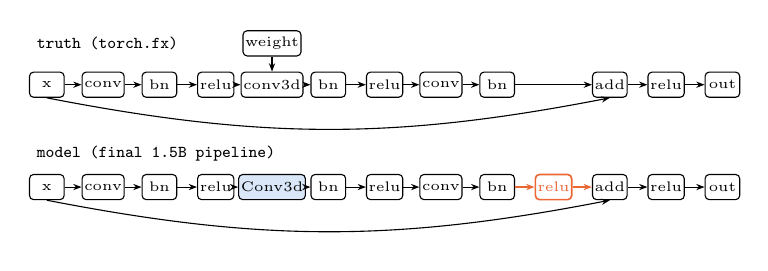
\begin{tikzpicture}[x=7.15mm, y=5mm, sm/.style={fx, font=\fontsize{4.9}{5.5}\selectfont, inner sep=0.8pt, minimum width=4.4mm, minimum height=3.2mm}]
\node[font=\demofont, anchor=west] at (-0.35,1.05) {truth (torch.fx)};
\foreach \i/\l in {0/x,1/conv,2/bn,3/relu,4/conv3d,5/bn,6/relu,7/conv,8/bn,10/add,11/relu,12/out}
  \node[sm] (t\i) at (\i,0) {\l};
\node[sm] (tw) at (4,1.05) {weight};
\foreach \a/\b in {0/1,1/2,2/3,3/4,4/5,5/6,6/7,7/8,8/10,10/11,11/12} \draw[ar] (t\a) -- (t\b);
\draw[ar] (tw) -- (t4); \draw[ar] (t0.south) to[bend right=11] (t10.south);
\node[font=\demofont, anchor=west] at (-0.35,-1.75) {model (final 1.5B pipeline)};
\foreach \i/\l in {0/x,1/conv,2/bn,3/relu,5/bn,6/relu,7/conv,8/bn,10/add,11/relu,12/out}
  \node[sm] (m\i) at (\i,-2.6) {\l};
\node[sm, fill=tagc!18] (m4) at (4,-2.6) {Conv3d};
\node[sm, draw=hiec, text=hiec, line width=0.6pt] (m9) at (9,-2.6) {relu};
\foreach \a/\b in {0/1,1/2,2/3,3/4,4/5,5/6,6/7,7/8,10/11,11/12} \draw[ar] (m\a) -- (m\b);
\draw[ar, draw=hiec, line width=0.6pt] (m8) -- (m9); \draw[ar, draw=hiec, line width=0.6pt] (m9) -- (m10);
\draw[ar] (m0.south) to[bend right=11] (m10.south);
\end{tikzpicture}
\captionof{figure}{Closest of the 17 unseen \tg{D4}, a video ResNet block (MC3): right but for one invented ReLU
(orange). Blue: a 3D conv as one layer; \texttt{torch.fx} writes weight + \texttt{conv3d}, the same computation.}
\end{minipage}
\end{multicols}

\begin{center}
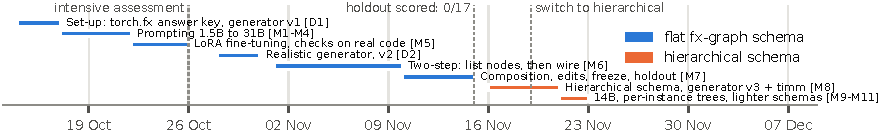
\includegraphics[width=\textwidth]{figures/fig2_gantt.pdf}
\captionof{figure}{Workflow, 14 Oct -- 22 Nov. Tags point to the data (D), methods (M) and results (R) below.}
\end{center}
\vspace{-7pt}

\begin{multicols}{2}
\sect{2\quad Data: why we generated our own}
\begin{itemize}
\item Training needs thousands of (code, graph) pairs; real model code is a few hundred files of the same
families. So we wrote \textbf{program generators}, answered by \texttt{torch.fx}.
\item The generator grew in steps: \textbf{v1} small programs in 4 tiers (chains, loops, branches, blocks)
$\rightarrow$ tiers 5--6 in library style (helper classes, containers) $\rightarrow$ \textbf{v2} adds the
torchvision habits behind our misses.
\item \textbf{Then we changed the answer format} (19 Nov, Sec.~3, Fig.~3c) and wrote \textbf{v3} for it: whole
networks (stages, repeats, configuration tables), plus 177 real \texttt{timm}~[6] models.
\item \textbf{D3 vs D4}: both real torchvision code. D3 we looked at while developing (we read its mistakes and
changed data and prompts), so its score is optimistic. D4, from 10 other families, nobody looked at; scored once, at
the end: the honest test.
\item \textbf{Foreshadowing:} the model learns the generator's \emph{house style}; what it never showed
(library layers, flags, constructor arithmetic) it never learned
\tg{R2}\tg{R4}\tg{R5}.
\end{itemize}
\end{multicols}
\vspace{-2pt}
\begin{center}
\scriptsize
\captionof{table}{Data sets. Graph size = nodes in the \texttt{torch.fx} graph, median (range).}
\begin{tabularx}{\textwidth}{@{}lXlll@{}}
\toprule
Tag & What it is & Programs & Graph size & Role\\
\midrule
\tg{D1} & Generated, tiers 1--4 (generator v1) & 1{,}280 train, 40 test & 11 (7--25) & the basic skill\\
\tg{D2} & Generated, tiers 5--6, library style (v1, then v2) & 640 train & 33 (8--119) & real-looking training code\\
\tg{D3} & Real torchvision~[5]: 18 blocks + 3 small networks & 21 & 14 (9--71) & development (``dev'')\\
\tg{D4} & Real torchvision, 10 families never looked at (\emph{holdout}) & 17 & 16 (9--159) & locked, scored once\\
\tg{D5} & Edits of D1 test programs: 69 change the graph, 124 do not & 193 & 12 (5--19) & does it follow the code?\\
\tg{D6} & Hier.\ training: v3 (1{,}350) + tiers 1--4 (283) + \texttt{timm} (177) & 1{,}810 & nets 131 (22--2{,}684) & training\\
\tg{D7} & Hierarchical dev: D3's 21 blocks + 30 whole torchvision networks & 51 & nets 177 (24--548) & development\\
\tg{D8} & Hierarchical generated test (v3): 24 blocks + 51 networks & 75 & nets 109 (29--352) & generated test\\
\tg{D9} & Hierarchical locked sets: unseen torchvision families + \texttt{timm} & 15 + 6 & up to 1{,}902 & not yet scored\\
\bottomrule
\end{tabularx}
\end{center}

% ------------------------------------------------------------------ demo: one program, both answers
\noindent\begin{minipage}{\textwidth}
\noindent\begin{minipage}[t]{0.335\textwidth}
{\footnotesize\textbf{(a) The input: PyTorch code}}\par\vspace{2pt}
\begin{lstlisting}
class Block(nn.Module):
    def __init__(self, c):
        super().__init__()
        self.conv = nn.Conv2d(c, c, 3, padding=1)
        self.bn = nn.BatchNorm2d(c)
    def forward(self, x):
        y = self.bn(self.conv(x))
        return torch.relu(x + y)

class Net(nn.Module):
    def __init__(self, c=8, depth=2):
        super().__init__()
        self.stem = nn.Conv2d(3, c, 3, padding=1)
        self.blocks = nn.Sequential(
            *[Block(c) for _ in range(depth)])
        self.head = nn.Linear(c, 10)
    def forward(self, x):
        x = self.blocks(self.stem(x))
        return self.head(x.mean((2, 3)))
\end{lstlisting}
\end{minipage}\hfill
\begin{minipage}[t]{0.645\textwidth}
{\footnotesize\textbf{(b) Flat format \tg{M1}--\tg{M7}: the \texttt{torch.fx} graph, 13 nodes}}\par\vspace{3pt}
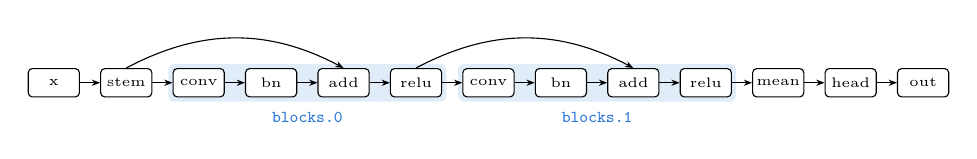
\begin{tikzpicture}[x=9.2mm]
\foreach \i/\l in {0/x,1/stem,2/conv,3/bn,4/add,5/relu,6/conv,7/bn,8/add,9/relu,10/mean,11/head,12/out}
  \node[fx] (n\i) at (\i,0) {\l};
\foreach \a/\b in {0/1,1/2,2/3,3/4,4/5,5/6,6/7,7/8,8/9,9/10,10/11,11/12} \draw[ar] (n\a) -- (n\b);
\draw[ar] (n1.north) to[bend left=28] (n4.north);
\draw[ar] (n5.north) to[bend left=28] (n8.north);
\begin{scope}[on background layer]
\node[fit=(n2)(n5), inner sep=1.5pt, fill=tagc!14, rounded corners=2pt, label={[font=\demofont, text=tagc]below:blocks.0}] {};
\node[fit=(n6)(n9), inner sep=1.5pt, fill=tagc!14, rounded corners=2pt, label={[font=\demofont, text=tagc]below:blocks.1}] {};
\end{scope}
\end{tikzpicture}\par\vspace{1pt}
{\footnotesize\textbf{(c) Hierarchical format \tg{M8}: a module tree + one small wiring graph per class}}\par\vspace{2pt}
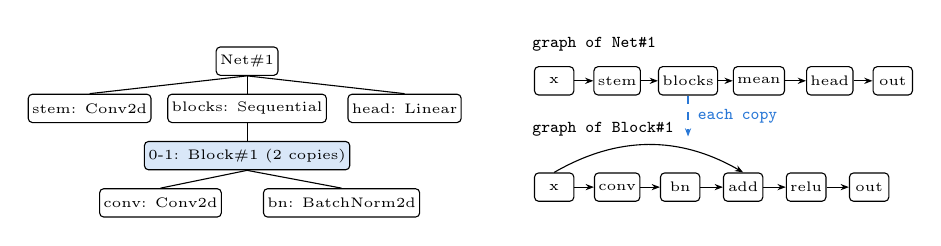
\begin{tikzpicture}[x=1mm, y=1mm, tn/.style={fx, minimum width=0pt}]
\node[tn] (net) at (19,0) {Net\#1};
\node[tn] (stem) at (-1,-6) {stem: Conv2d};
\node[tn] (blk) at (19,-6) {blocks: Sequential};
\node[tn] (head) at (39,-6) {head: Linear};
\node[tn, fill=tagc!18] (rep) at (19,-12) {0-1: Block\#1 (2 copies)};
\node[tn] (cv) at (8,-18) {conv: Conv2d};
\node[tn] (bnn) at (31,-18) {bn: BatchNorm2d};
\foreach \c in {stem,blk,head} \draw (net.south) -- (\c.north);
\draw (blk.south) -- (rep.north); \draw (rep.south) -- (cv.north); \draw (rep.south) -- (bnn.north);
\node[font=\demofont, anchor=west] at (54,2.2) {graph of Net\#1};
\foreach \i/\l/\p in {0/x/58,1/stem/66,2/blocks/75,3/mean/84,4/head/93,5/out/101}
  \node[fx, minimum width=5mm] (g\i) at (\p,-2.5) {\l};
\foreach \a/\b in {0/1,1/2,2/3,3/4,4/5} \draw[ar] (g\a) -- (g\b);
\node[font=\demofont, anchor=west] at (54,-8.6) {graph of Block\#1};
\foreach \i/\l/\p in {0/x/58,1/conv/66,2/bn/74,3/add/82,4/relu/90,5/out/98}
  \node[fx, minimum width=5mm] (h\i) at (\p,-16) {\l};
\foreach \a/\b in {0/1,1/2,2/3,3/4,4/5} \draw[ar] (h\a) -- (h\b);
\draw[ar] (h0.north) to[bend left=30] (h3.north);
\draw[ar, dashed, draw=tagc] (g2.south) -- ++(0,-5.2) node[midway, right, font=\demofont, text=tagc] {each copy};
\end{tikzpicture}
\end{minipage}
\captionof{figure}{Demo: one program, both formats (real answer-key output). (b) repeats every block, so it grows
with depth. (c) The tree says what is inside what and how many copies (\texttt{0-1: Block\#1}); each class is wired once.}
\end{minipage}
\vspace{-2pt}

\begin{multicols}{2}
\sect{3\quad Methods and approaches}
Models: Qwen2.5-Coder~[3] 1.5B--14B, Gemma 31B; LoRA~[2] (small add-on weights) on free Kaggle T4s.
\textbf{Exact} = same operations wired the same way as \texttt{torch.fx} (labelled graph isomorphism);
\textbf{lenient} also forgives notation (Table~1).

{\emph{Flat format -- the whole graph, Fig.~3b:}}
\begin{itemize}[label={},leftmargin=3.25em,labelsep=0pt,labelwidth=0pt,itemindent=-3.25em]
\item \makebox[3.25em][l]{\tg{M1}}\textbf{Zero-shot}: the code and the format rules only.
\item \makebox[3.25em][l]{\tg{M2}}\textbf{Few-shot}: + worked examples from the training split.
\item \makebox[3.25em][l]{\tg{M3}}\textbf{Chain of thought}: ``think step by step'' first~[4].
\item \makebox[3.25em][l]{\tg{M4}}\textbf{Chain of simulation}: track each variable's node~[7].
\item \makebox[3.25em][l]{\tg{M5}}\textbf{LoRA fine-tuning} (1.5B): whole graph in one go.
\item \makebox[3.25em][l]{\tg{M6}}\textbf{Two-step}: nodes first, then edges naming variables.
\item \makebox[3.25em][l]{\tg{M7}}\textbf{Composition}: one model lists, another wires.
\end{itemize}
\sub{The second format, and why (19 Nov)}
\begin{itemize}
\item Whole real networks are long in the flat format (median 177 nodes, up to 548; \texttt{timm} up to
2{,}684), every repeated block written out again: too long for a 1.5B to write, or to train on with a T4.
\item So we split the answer (Fig.~3c): a \textbf{tree} of modules (what is inside what, how many copies) and a
small \textbf{wiring graph per class} ($\le$27 nodes), each written once. Repeats become a count; wiring stays local.
\item Right only if the tree and every class graph are. New cost: the tree needs what the constructor builds \tg{R5}.
\end{itemize}
\begin{itemize}[label={},leftmargin=3.25em,labelsep=0pt,labelwidth=0pt,itemindent=-3.25em]
\item \makebox[3.25em][l]{\tg{M8}}\textbf{Tree + class graphs}: tree, then wiring; tuned 1.5B.
\item \makebox[3.25em][l]{\tg{M9}}\textbf{Prompted 14B} on M8, with 2 worked examples.
\item \makebox[3.25em][l]{\tg{M10}}\textbf{Per-instance trees}: one call per module, joined by code.
\item \makebox[3.25em][l]{\tg{M11}}\textbf{Lighter formats}: same replies, scored for less.
\end{itemize}

\sect{4\quad Results}
\sub{\tg{R1} Prompting: size decides it \tg{M1}--\tg{M4} on \tg{D1}}
\begin{itemize}
\item Right topology by size: 1.5B 5\%, 7B 25\%, 14B 60\%, 31B 93\%. Simulation \tg{M4} is best on the hardest tiers (14/20 vs 8/20 zero-shot) but breaks on nested containers;
``think step by step'' \tg{M3} is worst (24/40).
\end{itemize}

\sub{\tg{R2} Fine-tuning: perfect at home, lost on real code \tg{M5}}
\begin{itemize}
\item The 1.5B after $\sim$1.5\,h of LoRA: 40/40 on generated test code \tg{D1}, but \textbf{0/21} on real
torchvision \tg{D3}. It draws chains (Fig.~4). It learned our generator, not the rule.
\end{itemize}
\noindent\begin{minipage}{\columnwidth}\centering
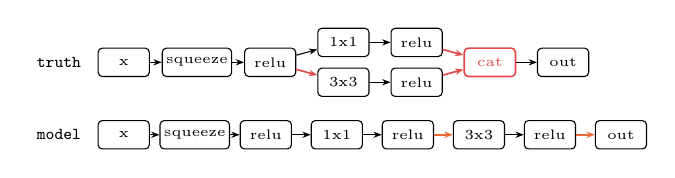
\begin{tikzpicture}[x=9.3mm, y=4.6mm]
\node[font=\demofont, anchor=east] at (-0.45,0) {truth};
\node[fx] (a0) at (0,0) {x}; \node[fx] (a1) at (1,0) {squeeze}; \node[fx] (a2) at (2,0) {relu};
\node[fx] (a3) at (3,0.55) {1x1}; \node[fx] (a4) at (4,0.55) {relu};
\node[fx] (a5) at (3,-0.55) {3x3}; \node[fx] (a6) at (4,-0.55) {relu};
\node[fx, draw=bad, text=bad, line width=0.6pt] (a7) at (5,0) {cat}; \node[fx] (a8) at (6,0) {out};
\foreach \a/\b in {0/1,1/2,2/3,3/4,5/6,7/8} \draw[ar] (a\a) -- (a\b);
\draw[ar, draw=bad, line width=0.6pt] (a2) -- (a5); \draw[ar, draw=bad, line width=0.6pt] (a4) -- (a7);
\draw[ar, draw=bad, line width=0.6pt] (a6) -- (a7);
\node[font=\demofont, anchor=east] at (-0.45,-2) {model};
\foreach \i/\l in {0/x,1/squeeze,2/relu,3/1x1,4/relu,5/3x3,6/relu,7/out}
  \node[fx] (b\i) at (\i*0.97,-2) {\l};
\foreach \a/\b in {0/1,1/2,2/3,3/4,5/6} \draw[ar] (b\a) -- (b\b);
\draw[ar, draw=hiec, line width=0.6pt] (b4) -- (b5); \draw[ar, draw=hiec, line width=0.6pt] (b6) -- (b7);
\end{tikzpicture}
\captionof{figure}{SqueezeNet's Fire block \tg{D3}. Truth: two parallel branches joined by \texttt{cat}. The
fine-tuned 1.5B chains them and drops \texttt{cat} (red: missed; orange: invented).}
\end{minipage}\vspace{2pt}

\sub{\tg{R3} Real-looking data, new formats \tg{M6}\tg{M7} (Table~1)}
\begin{itemize}
\item Training also on library-style code \tg{D2}: real blocks \tg{D3} 0 $\rightarrow$ \textbf{7/21} -- the
largest gain. Patching the generator on our own misses (v2) kept 7/21; we stopped, as that fits the dev set.
\item \textbf{The task splits in two.} The best lister names the right nodes on 15/21 but wires by listing order;
given the true nodes, a tuned 1.5B wirer is right on 16/21. Joined: \textbf{11/21}; 13/21 with the 14B wirer
(vs 7 alone, exact McNemar $p=0.03$).
\item \textbf{Edits \tg{D5}}: on edits that change the graph (e.g.\ \texttt{x + y} $\rightarrow$ \texttt{x + z}),
one-step returns the \emph{old} graph 57\% of the time, two-step 20\% ($p\approx4\times10^{-7}$); right 25\% vs 68\%.
\end{itemize}

\sub{\tg{R4} The locked test: 0/17 for every system \tg{D4}}
\begin{itemize}
\item Scored once, protocol fixed in advance: 0/17 (95\% interval 0--18\%), lenient too; not one node list right.
\item 13 of the 17 use torchvision layers whose code is \emph{not in the prompt} (e.g.\ \texttt{Conv2dNormActivation},
which \texttt{torch.fx} opens into conv $\rightarrow$ norm $\rightarrow$ activation); configuration flags decide
which branches run; 3D convolutions were never trained on (Fig.~1).
\end{itemize}

\sub{\tg{R5} Hierarchical: the tree is the bottleneck \tg{M8}\tg{D6}--\tg{D8}}
\begin{itemize}
\item (Fig.~5a) Generated test: 45/75 right; real blocks 9/21 (as before); real networks \textbf{0/30}.
\item Given the true tree, the same model gets 10/30 real networks right (0 $\rightarrow$ 10, $p=0.002$):
wiring partly works, writing the tree fails.
\item Why: the model must \emph{run the constructor in its head} (loop counts, computed widths, conditions).
Generated vs real networks: modules missing 2\% vs 20\%, settings wrong 6\% vs 37\%; e.g.\ ResNet-50's last
stage given 4 blocks (true: 3).
\end{itemize}

\sub{\tg{R6} Bigger model, less output \tg{M9}--\tg{M11} (Fig.~5b)}
\begin{itemize}
\item Prompted 14B: trees no better (networks 0/30; 2/30 lenient); wiring worse than the tuned 1.5B
(13 vs 26 of 51, true tree given).
\item Per-instance trees \tg{M10}: trained, not yet scored.
\item Asking for less: with class graphs only (S0: Fig.~3c without the tree), the same replies get \textbf{9/30}
real networks right, with 8$\times$ shorter output; found after seeing results, so descriptive until scored once
on \tg{D9}.
\end{itemize}

\sect{5\quad Conclusion}
\begin{itemize}
\item \textbf{Not achieved}: no unseen real network drawn exactly right, in either format.
\item \textbf{What holds}: the task splits into listing nodes and wiring them; wiring is learnable, listing (or
tree building) is the bottleneck; naming variables makes replies follow code edits.
\item \textbf{Why}: the generator was the ceiling -- real code relies on library layers, configuration and
constructor arithmetic it never showed.
\item \textbf{Next}: imported layers' code in the prompt; more real training code; repeat counts and widths
worked out before the tree; score S0 once on \tg{D9}.
\end{itemize}
\end{multicols}

\begin{center}
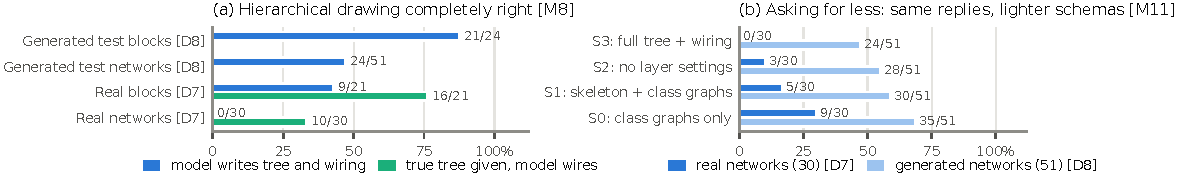
\includegraphics[width=\textwidth]{figures/fig4_hier.pdf}
\captionof{figure}{Hierarchical format. (a) Right drawings; aqua: true tree given \tg{R5}. (b) Same replies, lighter formats S3 to S0 \tg{R6}.}
\end{center}
\vspace{-9pt}
{\fontsize{5.3}{6}\selectfont\textbf{References.}
[1] James K. Reed, Zachary DeVito, Horace He and others. torch.fx: Practical Program Capture and Transformation for Deep Learning in Python, MLSys, 2022. \url{https://arxiv.org/abs/2112.08429}
[2] Edward J. Hu, Yelong Shen, Phillip Wallis and others. LoRA: Low-Rank Adaptation of Large Language Models, ICLR, 2022. \url{https://arxiv.org/abs/2106.09685}
[3] Binyuan Hui, Jian Yang, Zeyu Cui and others. Qwen2.5-Coder Technical Report, arXiv, 2024. \url{https://arxiv.org/abs/2409.12186}
[4] Jason Wei, Xuezhi Wang, Dale Schuurmans and others. Chain-of-Thought Prompting Elicits Reasoning in Large Language Models, NeurIPS, 2022. \url{https://arxiv.org/abs/2201.11903}
[5] TorchVision maintainers and contributors. \url{https://github.com/pytorch/vision}. Accessed on: 22nd November, 2026.
[6] Ross Wightman. \url{https://github.com/huggingface/pytorch-image-models}. Accessed on: 22nd November, 2026.
[7] Maxwell Nye, Anders Johan Andreassen, Guy Gur-Ari and others. Show Your Work: Scratchpads for Intermediate Computation with Language Models, arXiv, 2021. \url{https://arxiv.org/abs/2112.00114}
\quad\textbf{Code:} \url{https://github.com/Rao-Adarsh/graphArt_LM}\par}
\end{document}
